% SC4053 --- Chapter 3: Transactions, UTXO and Account Models (0->100)
\chapter{Transactions, UTXO and the Account Model}\label{ch:transactions}

\begin{quote}
\emph{``A transaction is not a row in a spreadsheet; it is a transformation of ownership that must conserve value and never double-spend.''} --- This chapter traces how value moves and why two competing models (UTXO vs accounts) exist.
\end{quote}

\noindent\fbox{\parbox{\dimexpr\linewidth-2\fboxsep-2\fboxrule}{%
\textbf{From zero: no transaction background assumed.} We start from a paper cheque (who pays whom, what prevents photocopying?) and build the digital equivalents. We define inputs/outputs, UTXO graphs and account nonces from scratch, then verify real transactions with Python.}}
\vspace{0.4em}

\section*{Learning Outcomes}
After this chapter you will be able to:
\begin{enumerate}[label=(L\arabic*)]
    \item define a transaction, input, output and script; explain conservation;
    \item construct and validate a UTXO graph and detect double-spends;
    \item contrast UTXO (Bitcoin) with account model (Ethereum) on state, parallelism and privacy;
    \item explain nonce, gas price, fee and replay protection (chain-id);
    \item simulate a mempool that orders by fee rate and packs a block.
\end{enumerate}

% ============================================================
\section{Transactions as Value Flow}\label{sec:tx-flow}
A \emph{transaction} $tx$ maps old coins to new coins. Each transaction has a list of \emph{inputs} (references to coins being spent) and \emph{outputs} (new coins being created), plus signatures proving ownership of the inputs.

Two rules must hold for validity:
\begin{enumerate}[label=(\roman*)]
    \item \emph{No double-spend}: each input must reference an unspent coin that exists and has not been spent before.
    \item \emph{Conservation}: $\sum \text{inputs} \ge \sum \text{outputs}$; the difference is the fee (miner/validator reward).
\end{enumerate}
If any rule breaks, the transaction is invalid regardless of signatures.

% ============================================================
\section{The UTXO Model}\label{sec:utxo}
Bitcoin's \emph{Unspent Transaction Output} model treats coins as discrete, consumable objects. The ledger state is the set $\mathcal{U}$ of UTXOs. Spending consumes UTXOs atomically and creates new ones.

\begin{definition}[UTXO]\label{def:utxo}
A UTXO is a triple $(txid, index, value, scriptPubKey)$ where $scriptPubKey$ is the spending condition (e.g., ``pay to public key $pk$''). The set $\mathcal{U}$ contains exactly the UTXOs whose outputs have not been consumed as inputs elsewhere.
\end{definition}

\begin{figure}[h]\centering
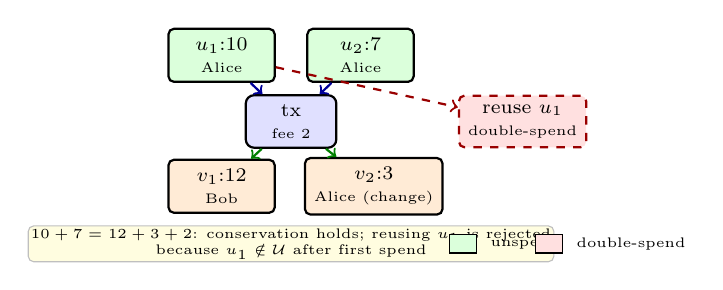
\begin{tikzpicture}[scale=0.84, every node/.style={font=\scriptsize},
  utxo/.style={draw,rounded corners=2pt,minimum width=1.35cm,minimum height=0.52cm,align=center,thick},
  txb/.style={draw,rounded corners=3pt,fill=blue!12,minimum width=1.15cm,minimum height=0.62cm,align=center,thick}]
\node[utxo,fill=green!14] (u1) at (0,2.10) {$u_1$:10\\ \tiny Alice};
\node[utxo,fill=green!14] (u2) at (2.10,2.10) {$u_2$:7\\ \tiny Alice};
\node[txb] (tx) at (1.05,1.10) {tx\\ \tiny fee 2};
\draw[->,thick,blue!60!black] (u1)--(tx); \draw[->,thick,blue!60!black] (u2)--(tx);
\node[utxo,fill=orange!16] (v1) at (0,0.12) {$v_1$:12\\ \tiny Bob};
\node[utxo,fill=orange!16] (v2) at (2.30,0.12) {$v_2$:3\\ \tiny Alice (change)};
\draw[->,thick,green!50!black] (tx)--(v1); \draw[->,thick,green!50!black] (tx)--(v2);
\node[utxo,fill=red!12,draw=red!60!black,dashed] (bad) at (4.55,1.10) {reuse $u_1$\\ \tiny double-spend};
\draw[->,thick,red!60!black,dashed] (u1) -- (bad);
\node[font=\tiny,fill=yellow!12,draw=gray!50,rounded corners=2pt,inner sep=1pt,align=center] at (1.05,-0.75) {$10+7 = 12+3+2$: conservation holds; reusing $u_1$ is rejected\\because $u_1\notin\mathcal{U}$ after first spend};
% legend
\node[draw,fill=green!14,minimum width=0.34cm,minimum height=0.20cm] at (3.65,-0.75) {}; \node[font=\tiny,anchor=west] at (3.92,-0.75) {unspent};
\node[draw,fill=red!12,minimum width=0.34cm,minimum height=0.20cm] at (4.95,-0.75) {}; \node[font=\tiny,anchor=west] at (5.22,-0.75) {double-spend};
\end{tikzpicture}
\caption{UTXO flow: Alice consumes $u_1,u_2$ (10+7) to pay Bob 12, reclaim 3 as change, and leave fee 2. Any attempt to reuse $u_1$ (red, dashed) fails because the UTXO set no longer contains it. The graph is a DAG.}
\label{fig:utxo}
\end{figure}

UTXO is inherently parallelisable: disjoint input sets do not conflict. It also helps privacy (new addresses per output) but makes stateful contracts harder (no notion of ``account balance'').

\begin{lstlisting}[language=Python]
# UTXO validator (simplified)
utxo = {("tx0",0): {"value":10,"owner":"Alice"}, ("tx0",1): {"value":7,"owner":"Alice"}}
def validate(tx, utxo_set):
    ins = tx["inputs"]    # list of (txid, idx)
    outs = tx["outputs"]  # list of {"value":..., "owner":...}
    # (i) existence + no double-spend within tx
    assert len(set(ins)) == len(ins), "duplicate input in tx"
    total_in = 0
    for ref in ins:
        assert ref in utxo_set, f"missing/already spent {ref}"
        total_in += utxo_set[ref]["value"]
    total_out = sum(o["value"] for o in outs)
    assert total_in >= total_out, "creates money!"
    fee = total_in - total_out
    return fee

tx = {"inputs":[("tx0",0),("tx0",1)], "outputs":[{"value":12,"owner":"Bob"},{"value":3,"owner":"Alice"}]}
print("fee:", validate(tx, utxo))  # 2
# Double-spend attempt: reuse (tx0,0)
tx2 = {"inputs":[("tx0",0)], "outputs":[{"value":9,"owner":"Carol"}]}
# Simulate applying tx first
del utxo[("tx0",0)]; del utxo[("tx0",1)]
utxo[("tx1",0)] = {"value":12,"owner":"Bob"}; utxo[("tx1",1)] = {"value":3,"owner":"Alice"}
try: validate(tx2, utxo)
except AssertionError as e: print("rejected:", e)
\end{lstlisting}

% ============================================================
\section{The Account Model}\label{sec:account}
Ethereum uses \emph{accounts}: each address maps to $(balance, nonce, codeHash, storageRoot)$. A transaction is a state transition
\begin{equation}\label{eq:acct-tx}
\sigma_{t+1} = \Upsilon(\sigma_t, tx),\quad tx=(nonce, gasPrice, gasLimit, to, value, data, v,r,s).
\end{equation}
The \emph{nonce} is a per-sender counter preventing replay; $gasPrice\times gasUsed$ pays for computation.

\begin{figure}[h]\centering
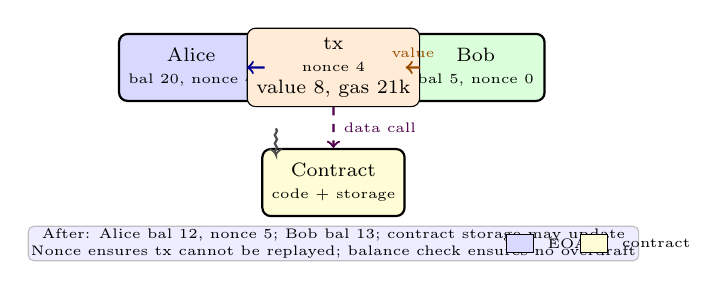
\begin{tikzpicture}[scale=0.86, every node/.style={font=\scriptsize},
  acct/.style={draw,rounded corners=3pt,minimum width=1.75cm,minimum height=0.85cm,align=center,thick}]
\node[acct,fill=blue!15] (a0) at (0,1.75) {Alice\\ \tiny bal 20, nonce 4};
\node[acct,fill=green!14] (b0) at (4.20,1.75) {Bob\\ \tiny bal 5, nonce 0};
\node[acct,fill=yellow!16] (c0) at (2.10,0.05) {Contract\\ \tiny code + storage};
\node[draw,fill=orange!16,rounded corners=3pt,minimum width=1.35cm,minimum height=0.62cm,align=center] (tx) at (2.10,1.75) {tx\\ \tiny nonce 4\\ value 8, gas 21k};
\draw[->,thick,blue!60!black] (a0)--(tx);
\draw[->,thick,orange!60!black] (tx)--(b0) node[midway,above,font=\tiny] {value};
\draw[->,thick,violet!60!black,dashed] (tx)--(c0) node[midway,right,font=\tiny] {data call};
% state transition arrow
\draw[->,thick,gray!60!black,decorate,decoration={snake,amplitude=0.4pt,segment length=3pt}] (1.25,0.85) -- (1.25,0.45);
\node[font=\tiny,fill=blue!7,draw=gray!50,rounded corners=2pt,inner sep=1pt,align=center] at (2.10,-0.85) {After: Alice bal 12, nonce 5; Bob bal 13; contract storage may update\\Nonce ensures tx cannot be replayed; balance check ensures no overdraft};
% legend
\node[draw,fill=blue!15,minimum width=0.34cm,minimum height=0.20cm] at (4.85,-0.85) {}; \node[font=\tiny,anchor=west] at (5.12,-0.85) {EOA};
\node[draw,fill=yellow!16,minimum width=0.34cm,minimum height=0.20cm] at (5.95,-0.85) {}; \node[font=\tiny,anchor=west] at (6.22,-0.85) {contract};
\end{tikzpicture}
\caption{Account-model transition: a signed transaction increments the sender nonce, moves value, and may call contract code. The global state $\sigma$ is a map address$\to$account.}
\label{fig:account-model}
\end{figure}

\begin{example}[Replay without chain-id]\label{ex:replay}
Alice signs $tx$ with nonce 4 on chain A. Without a chain-id in the signed data, an attacker can rebroadcast the same bytes on chain B where Alice also has funds and the same nonce is valid. EIP-155 fixes this by including $chainId$ in the hash that is signed.
\end{example}

\begin{lstlisting}[language=Python]
# Account nonce + replay protection (simplified)
state = {"Alice":{"balance":20,"nonce":4}, "Bob":{"balance":5,"nonce":0}}
def apply_account_tx(state, tx, chain_id=1):
    # tx: {from, to, value, nonce, gas_price, gas_limit, chain_id, sig_ok}
    assert tx["sig_ok"], "bad signature"
    assert tx["chain_id"] == chain_id, "wrong chain -- replay!"
    s = state[tx["from"]]
    assert tx["nonce"] == s["nonce"], f"bad nonce expected {s['nonce']}"
    cost = tx["value"] + tx["gas_price"]*tx["gas_limit"]
    assert s["balance"] >= cost, "insufficient funds"
    # apply
    s["balance"] -= cost; s["nonce"] += 1
    state[tx["to"]]["balance"] += tx["value"]
    return state

tx = {"from":"Alice","to":"Bob","value":8,"nonce":4,"gas_price":0,"gas_limit":0,"chain_id":1,"sig_ok":True}
print(apply_account_tx(state, tx))
# Replaying same tx fails: nonce now 5
try: apply_account_tx(state, tx)
except AssertionError as e: print("replay rejected:", e)
\end{lstlisting}

% ============================================================
\section{Mempool, Fees and Block Packing}\label{sec:mempool}
Users broadcast transactions to a \emph{mempool} (pending set). Validators pack blocks greedily by \emph{fee rate} ($\text{gasPrice}$ or tip) to maximise revenue, subject to block gas limit.

\begin{figure}[h]\centering
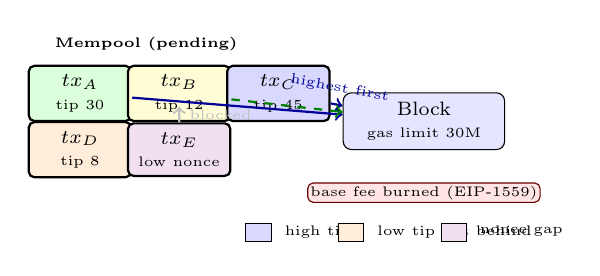
\begin{tikzpicture}[scale=0.84, every node/.style={font=\scriptsize},
  tx/.style={draw,rounded corners=2pt,minimum width=1.30cm,minimum height=0.50cm,align=center,thick}]
\node[font=\tiny\bfseries] at (1.35,2.55) {Mempool (pending)};
\node[tx,fill=green!14] (t1) at (0.35,1.80) {$tx_A$\\ \tiny tip 30};
\node[tx,fill=yellow!16] (t2) at (1.85,1.80) {$tx_B$\\ \tiny tip 12};
\node[tx,fill=blue!15] (t3) at (3.35,1.80) {$tx_C$\\ \tiny tip 45};
\node[tx,fill=orange!15] (t4) at (0.35,0.95) {$tx_D$\\ \tiny tip 8};
\node[tx,fill=violet!12] (t5) at (1.85,0.95) {$tx_E$\\ \tiny low nonce};
\draw[->,thick,gray!50] (t5) -- (1.85,1.60) node[midway,right,font=\tiny] {blocked};
\node[draw,fill=blue!10,rounded corners=3pt,minimum width=2.05cm,minimum height=0.68cm,align=center] (blk) at (5.55,1.38) {Block\\ \tiny gas limit 30M};
\draw[->,thick,blue!60!black] (t3)--(blk) node[midway,above,font=\tiny,sloped] {highest first};
\draw[->,thick,blue!60!black] (t1)--(blk);
\draw[->,thick,green!50!black,dashed] (t2)--(blk);
\node[font=\tiny,fill=red!10,draw=red!40!black,rounded corners=2pt,inner sep=1pt] at (5.55,0.30) {base fee burned (EIP-1559)};
% legend
\node[draw,fill=blue!15,minimum width=0.32cm,minimum height=0.18cm] at (3.05,-0.30) {}; \node[font=\tiny,anchor=west] at (3.30,-0.30) {high tip};
\node[draw,fill=orange!15,minimum width=0.32cm,minimum height=0.18cm] at (4.45,-0.30) {}; \node[font=\tiny,anchor=west] at (4.70,-0.30) {low tip left behind};
\node[draw,fill=violet!12,minimum width=0.32cm,minimum height=0.18cm] at (6.00,-0.30) {}; \node[font=\tiny,anchor=west] at (6.25,-0.30) {nonce gap};
\end{tikzpicture}
\caption{Mempool ordering by tip (priority fee). Validators greedily fill the block; transactions with nonce gaps or below the base fee wait. EIP-1559 burns the base fee and only the tip goes to the validator.}
\label{fig:mempool}
\end{figure}

\begin{remark}[Fee markets]\label{rem:fee}
EIP-1559 introduced a protocol-computed \emph{base fee} that adjusts up/down by 12.5\% per block to target half-full blocks; users add a \emph{tip} to outbid others. This smooths fee spikes versus pure first-price auctions.
\end{remark}

Comparison table:

\begin{center}\small
\begin{tabular}{lcc}
\toprule
 & UTXO & Account \\
\midrule
State & set $\mathcal{U}$ & map $addr\to(bal,nonce,\dots)$ \\
Parallelism & easy (disjoint inputs) & harder (overlaps on same account)\\
Smart contracts & limited (script) & rich (Turing-complete via EVM)\\
Privacy & better (fresh addrs) & address reuse common\\
\bottomrule
\end{tabular}
\end{center}

% ============================================================
\section{Exercises}\label{sec:ch03-exercises}
\begin{enumerate}[label=E3.\arabic*, leftmargin=*, itemsep=0.6em]
    \item \textbf{UTXO trace.} Given $\mathcal{U}=\{a{:}5,b{:}3,c{:}8\}$, trace a transaction consuming $a,c$ to create $d{:}10$ (Bob) and change. What is the fee? Show the UTXO set before and after.
    \item \textbf{Double-spend hunt.} Two transactions both consume $a{:}5$. Explain why only one can be included and how the mempool/consensus resolves the conflict. What if they are in competing forks?
    \item \textbf{Account replay.} Alice has nonce 7. She signs $tx$ with nonce 7 on chain 1. Show step-by-step what happens if the same bytes are submitted on chain 2 where her nonce is also 7 and chain-id is not checked.
    \item \textbf{Fee estimator.} Write a Python function that, given a mempool list of $(gasUsed, tip)$ and a block gas limit, selects the revenue-maximising subset (knapsack) and compares it to greedy-by-tip order.
    \item \textbf{UTXO vs account.} A game needs per-player state (level, inventory). Argue why UTXO is awkward and how the account model's storage trie helps. Propose a UTXO workaround and its cost.
\end{enumerate}

\section*{Chapter Notes}
Bitcoin's transaction format in Nakamoto (2008) and BIP docs; UTXO set theory in Antonopoulos, \emph{Mastering Bitcoin} (O'Reilly, 2nd ed.); Ethereum account model and EIP-1559 in Wood, \emph{Yellow Paper} and ethereum.org specs; fee-market analysis in Roughgarden, ``Transaction fee mechanism design for the Ethereum blockchain'' (2021).
% End Ch03
